\documentclass[a4paper,9pt,twocolumn]{extarticle}
\usepackage[margin=1.2cm,top=0.9cm,bottom=0.85cm]{geometry}
\usepackage{graphicx,booktabs,xcolor,microtype,amsmath,amssymb}
\usepackage[T1]{fontenc}
\usepackage{mathptmx}
\usepackage[colorlinks=true,linkcolor=black,citecolor=black,urlcolor=blue]{hyperref}
\usepackage{titlesec}
\usepackage{caption}
\usepackage{enumitem}
\usepackage{fancyvrb}
\usepackage{tcolorbox}

\captionsetup{font=footnotesize,labelfont=bf,skip=2pt}
\titlespacing*{\section}{0pt}{5pt}{2pt}
\titlespacing*{\subsection}{0pt}{4pt}{1pt}
\titleformat{\section}{\normalfont\large\bfseries}{\thesection}{0.5em}{}
\titleformat{\subsection}{\normalfont\normalsize\bfseries}{\thesubsection}{0.5em}{}
\setlength{\parskip}{1.2pt}
\setlength{\abovedisplayskip}{3pt}
\setlength{\belowdisplayskip}{3pt}
\setlength{\textfloatsep}{6pt}
\setlength{\floatsep}{5pt}
\setlength{\intextsep}{5pt}
\setlist{nosep,leftmargin=1.1em}
\pagestyle{empty}

\newtcolorbox{prompt}[1]{colback=black!3,colframe=black!45,boxrule=0.3pt,
  left=3pt,right=3pt,top=2pt,bottom=2pt,arc=1pt,
  title={\scriptsize\bfseries #1},fonttitle=\scriptsize,
  coltitle=white,colbacktitle=black!55,boxsep=1pt}

\begin{document}

\twocolumn[
\begin{center}
{\Large\bfseries A hybrid local-LLM / classical / U-Net pipeline for
fluorescence-microscopy nucleus analysis}

\vspace{3pt}
{\normalsize Biomedical Image Analysis assignment --- modality: fluorescence
microscopy (DAPI-like stained nuclei)}
\end{center}
\vspace{6pt}
]

\section{Data, preprocessing and EDA}

The assigned dataset is a synthetic stained-nuclei set of 112 labelled
$256\times256$ RGB images (80 train / 20 validation / 12 unseen test) plus 4
corrupted test variants, with exact binary and instance ground truth. Images are
drawn from four density regimes --- \textit{sparse}, \textit{normal},
\textit{dense} and \textit{clustered} --- with 5--85 nuclei per image (mean 32.4)
and a mean foreground area fraction of 0.081.

Preprocessing is a single function shared by every downstream stage
(\texttt{common.load\_gray}): RGB $\rightarrow$ ITU-R 601-2 luma $\rightarrow$
$256\times256$ float32 in $[0,1]$. Class-conditional statistics (Fig.~1, right)
show mean nucleus intensity 0.255 against background 0.016 --- a clean bimodal
histogram, which is precisely why Otsu does so well later.

One choice deserves scrutiny. The stain is DAPI-like blue and luma weights blue
by only 0.0721, so grayscale conversion discards $\sim$93\% of the channel
carrying the signal (blue-channel foreground mean 0.734 vs 0.255 for luma). We
ablated it: Otsu was run on both conversions over the whole validation split and
mean Dice was \textbf{identical to four decimals} (0.9733), because luma
rescales nuclei and background noise together, preserving the contrast-to-noise
ratio that Otsu actually keys on. A preprocessing step that looks catastrophic
in absolute terms can be irrelevant to a scale-invariant algorithm --- but it is
not irrelevant to the U-Net (Section~\ref{sec:ext}).

\begin{figure}[t]
\centering
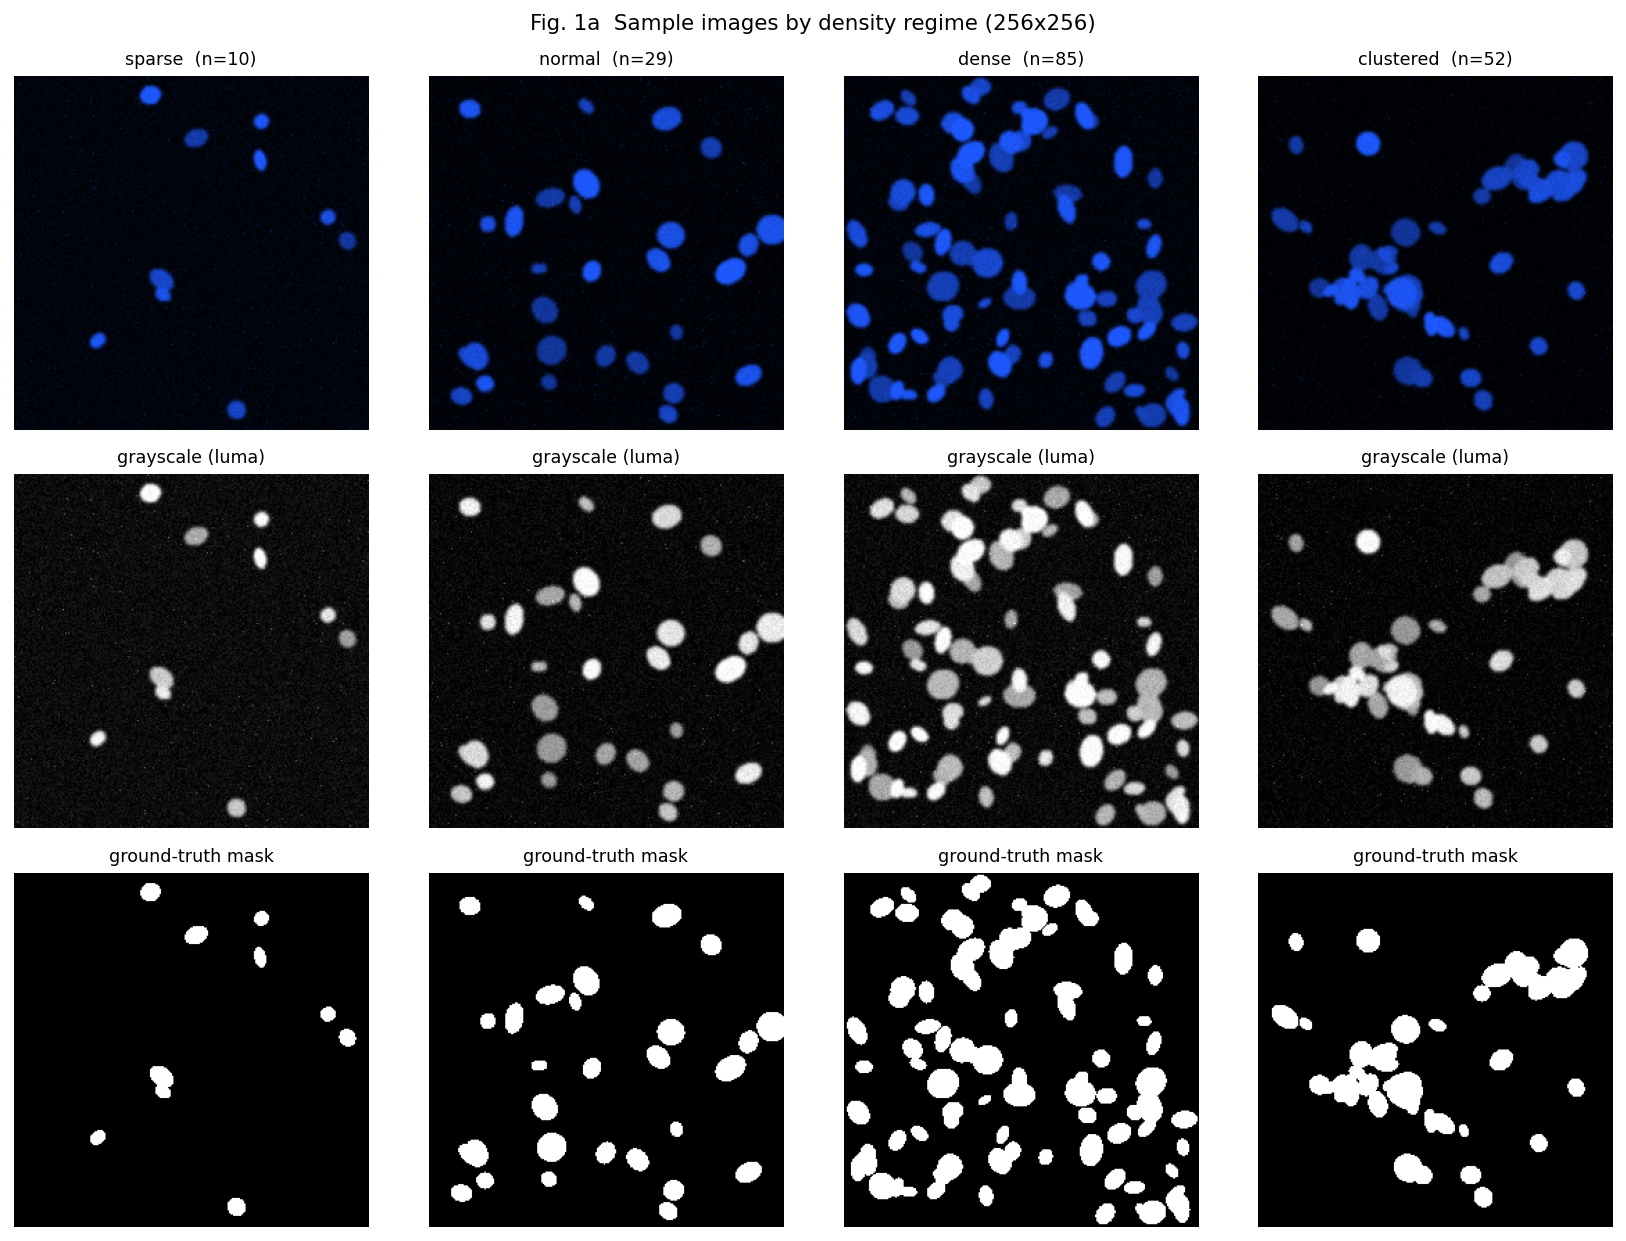
\includegraphics[width=0.82\linewidth]{../results/figures/fig1a_samples.png}\\[2pt]
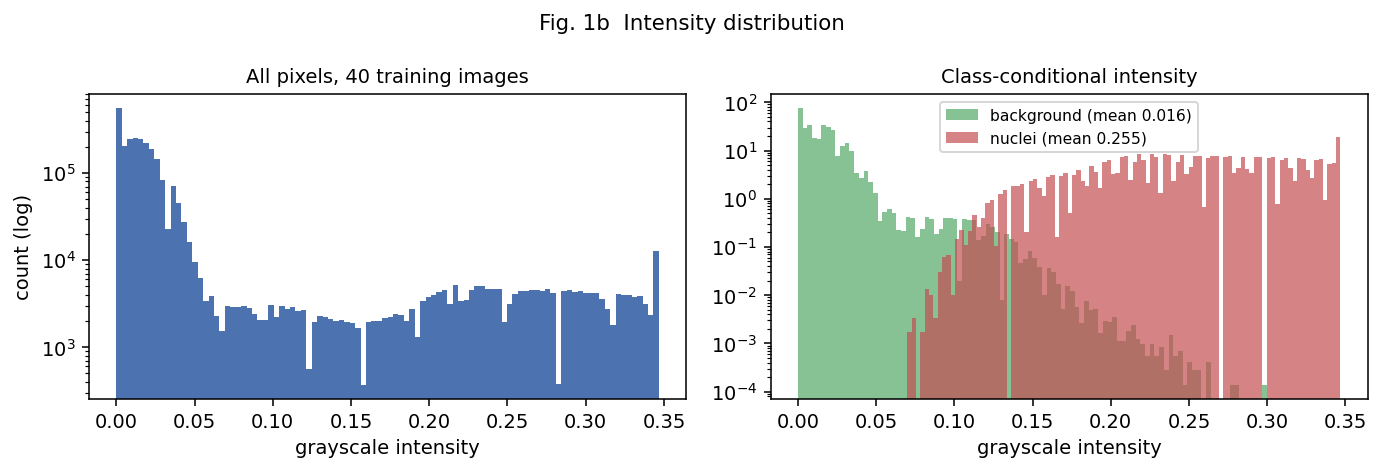
\includegraphics[width=\linewidth]{../results/figures/fig1b_histograms.png}
\caption{Sample images by density regime (RGB, luma grayscale, ground-truth
mask) and the intensity distribution over 40 training images. Foreground and
background are cleanly separated, which sets the difficulty level for every
later stage.}
\end{figure}

\section{Task 1 --- multimodal LLM description}

\begin{prompt}{Provenance of the LLM text in this report}
\scriptsize
The pipeline calls \texttt{llama3.2-vision} (image steps) and
\texttt{llama3.1} (text steps) through a local Ollama server. Where no Ollama
server is reachable, \texttt{src/llm.py} falls back to a documented rule-based
\emph{offline stub} so that the pipeline still runs end to end. \textbf{The runs
reported here used the offline stub}: every artefact is tagged
\texttt{"generator": "offline\_stub"} in \texttt{results/json/}. The stub is
\emph{not} a language model. All non-LLM results (EDA, Otsu, U-Net, metrics,
robustness, ablation) are genuine measurements and are unaffected. Re-running
the same scripts with Ollama up overwrites the LLM artefacts with real model
outputs; no code change is needed.
\end{prompt}

A representative image was selected reproducibly as the validation image whose
object count is closest to the dataset median (\texttt{val\_007}, 29 nuclei,
\textit{normal} density) and sent to the vision back-end. Two prompts were
compared.

\begin{prompt}{Naive prompt (baseline)}
\scriptsize\ttfamily What do you see in this medical image?
\end{prompt}

\begin{prompt}{Optimised structured prompt (Task 1)}
\scriptsize\ttfamily
You are a descriptive image-annotation assistant for a microscopy teaching
dataset. You are NOT a clinician and you must NOT diagnose, grade, stage, name a
disease, or suggest management.\\[2pt]
Describe ONLY what is directly visible in this image: staining pattern, object
shape, size and spacing, background, and technical image quality. Do not infer
patient information, do not name organs you cannot see, and do not invent scale
bars, magnification or units that are not shown.\\[2pt]
If a field cannot be determined from the pixels alone, you MUST answer exactly
"uncertain" rather than guessing. "uncertain" is a correct answer, not a
failure.\\[2pt]
Return ONE JSON object and nothing else -- no preamble, no markdown fence, no
commentary after the closing brace. Use exactly these keys:\\[2pt]
\{"modality": "<one of: fluorescence\_microscopy | brightfield\_microscopy |
histopathology | radiograph | uncertain>", "tissue\_type": "<short noun phrase,
or 'uncertain'>", "notable\_features": ["<3-6 short visual observations>"],
"image\_quality": "<one of: good | moderate | poor | uncertain>"\}
\end{prompt}

Four decisions do the work. (i) An explicit role and prohibition removes the
strongest attractor in the model's prior, which is to talk like a pathology
report. (ii) A closed vocabulary per field converts free text into a categorical
variable code can validate. (iii) ``\texttt{uncertain} is a correct answer''
licenses abstention; without it, refusing is off-distribution and the model
invents a value instead. (iv) ``no preamble, no markdown fence'' targets the
formatting failure that breaks automated parsing.

\textbf{Structured vs naive.} The harness scores every reply with the same
parser used downstream (\texttt{llm.extract\_json}, which tolerates markdown
fences and preamble and additionally requires all four keys). Over six
validation images the naive prompt yielded parseable, schema-complete JSON on
\textbf{0/6} and the structured prompt on \textbf{6/6}. The naive reply is
prose, so 0/6 is structural rather than incidental: no amount of retrying makes
free text machine-readable. The naive reply also drifts into clinical register,
volunteering phrases such as ``consistent with a hyperproliferative process''
and ``further evaluation by a pathologist is advised'' about an image whose
ground truth is 29 synthetic ellipses on a black field. Nothing in the pixels
supports either claim. (With the offline back-end this drift is emulated by
design; it is the documented failure mode of unconstrained medical VLM prompting
\cite{ji2023}, and the structured prompt is written to block it.)

\textbf{Repeated runs are not identical.} Running the structured prompt three
times at \texttt{temperature=0.8} with different seeds gave \textbf{3 distinct
responses out of 3}. The constrained fields agreed every time
(\texttt{modality}, \texttt{tissue\_type}, \texttt{image\_quality}) while the
free-text list \texttt{notable\_features} varied in content and ordering on
every run. That contrast is the practical finding, and it holds for any sampled
decoder: schema constraints buy reproducibility exactly where they are applied
and nowhere else. Setting \texttt{temperature=0} makes decoding greedy and
removes most of the variance, at the cost of hiding the model's uncertainty
rather than resolving it --- which is why the pipeline logs temperature, seed
and raw response for every call.

\section{Task 2 --- classical features, numbers-first LLM}

The classical route is Otsu thresholding, morphological cleanup (opening
$r{=}2$ to remove speckle, closing $r{=}2$, hole-fill $\leq64$\,px, discard
objects $<20$\,px), connected-component labelling and
\texttt{skimage.measure.regionprops\_table} (Fig.~2). For \texttt{val\_007} the
threshold was 0.129, giving Dice 0.973 / IoU 0.948 against ground truth and 19
labelled objects.

\begin{figure*}[t]
\centering
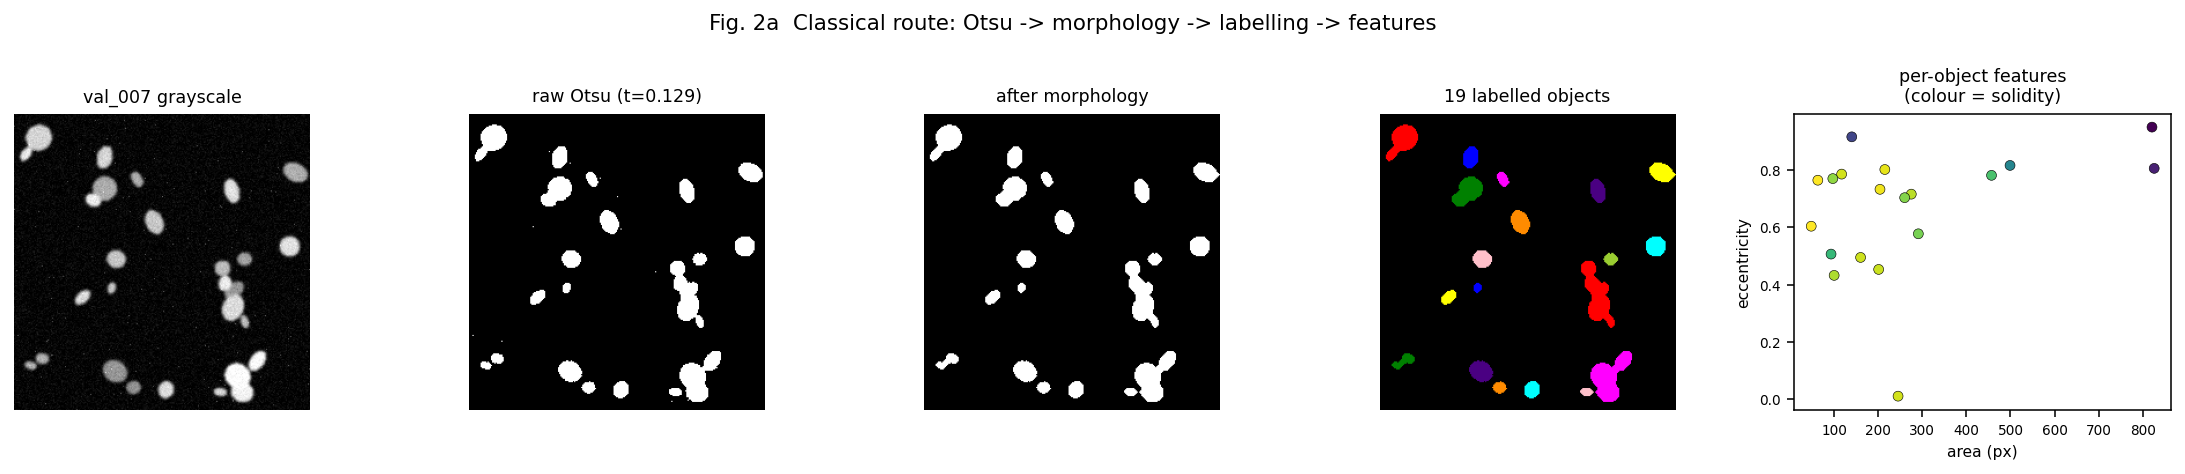
\includegraphics[width=0.97\textwidth]{../results/figures/fig2a_classical.png}
\caption{Classical route on \texttt{val\_007}: grayscale $\rightarrow$ raw Otsu
$\rightarrow$ morphological cleanup $\rightarrow$ connected components
$\rightarrow$ per-object features. The rightmost panel shows the area /
eccentricity / solidity structure that the LLM is later asked to summarise.
Several labelled ``objects'' are visibly two touching nuclei merged into one.}
\end{figure*}

The 19-object table is collapsed to 14 numbers (count, foreground fraction,
area mean/sd/median/range, equivalent diameter, eccentricity, solidity,
circularity, extent, object and background intensity), rendered as plain text
and passed to a local text model. \textbf{The model never sees the image.}

\begin{prompt}{Optimised numbers-first prompt (Task 2, abridged rules block)}
\scriptsize\ttfamily
You are interpreting a quantitative measurement table from an automated
microscopy image-analysis pipeline. You have NOT seen the image and you must not
pretend that you have: describe only what the numbers below support, and never
invent a colour, a stain, an artefact, a diagnosis or a count that is not in the
numbers.\\[2pt]
MEASUREMENTS\\
\{summary\}\\[2pt]
Interpretation rules (apply them literally, do not re-derive them):\\
\ \ density\_class\ \ \ \ : sparse if n\_objects < 15, normal if 15-34, dense if
35-59, clustered if >= 60 OR mean solidity < 0.90\\
\ \ shape\_regularity : regular if mean eccentricity < 0.65 and mean solidity
>= 0.95, irregular if mean eccentricity >= 0.80 or mean solidity < 0.90,
otherwise mixed\\
\ \ quality\_flag\ \ \ \ : ok if the foreground fraction is 0.01-0.35 and
n\_objects >= 3; otherwise review\\[2pt]
Respond with EXACTLY two parts and nothing else:\\
PARAGRAPH:\\
<one paragraph, 3-5 sentences, plain English, quoting the numbers you rely on.
Say "uncertain" wherever the table does not settle the question.>\\
JSON:\\
\{"n\_objects": <int>, "density\_class": "<sparse|normal|dense|clustered>",
"shape\_regularity": "<regular|mixed|irregular>", "quality\_flag": "<ok|review>"\}
\end{prompt}

Moving the thresholds into the prompt as literal rules is deliberate: it turns
the model from an estimator into a formatter, so its output is checkable by a
three-line function. The returned record for \texttt{val\_007} was

{\footnotesize\ttfamily\{"n\_objects": 19, "density\_class": "normal",
"shape\_regularity": "mixed", "quality\_flag": "ok"\}}

\noindent and the accompanying paragraph quotes the measured area
($269.1\pm223.4$\,px), eccentricity (0.664) and solidity (0.937), and states
explicitly that a solidity below 1.0 cannot distinguish a genuinely lobed
nucleus from two touching nuclei merged into one label. That hedge is not
politeness; it is the one place where the numbers genuinely under-determine the
answer, and the prompt's ``say uncertain'' clause is what surfaces it.

\textbf{Otsu quality across the validation split} was mean Dice 0.9733, IoU
0.9480, essentially flat across density regimes (0.971--0.974). The pixel
metrics conceal the real failure: Otsu detected on average 10.8 fewer objects
per image than ground truth, and on \textit{clustered} images it under-counted
by 27 (e.g. \texttt{val\_011}: 14 detected, 32 present). A binary mask simply
cannot represent the boundary between two touching nuclei, so every downstream
number derived from object identity --- count, mean area, density class --- is
biased, while Dice stays near 0.97.

\section{Task 3 --- U-Net segmentation}

The U-Net is deliberately small: base width 16, depth 3 (16/32/64, bottleneck
128), 482{,}449 parameters. A full-width U-Net \cite{ronneberger2015} has
$\sim$31\,M parameters, which on 80 training images would memorise the set
within a few epochs. Training used Adam ($10^{-3}$, cosine annealing), batch 8,
40 epochs, BCE+soft-Dice ($w{=}0.5$), and geometric augmentation only (flips,
$90^\circ$ rotations) because nuclei have no canonical orientation so these
transforms are exactly label-preserving. Training took 628\,s on two CPU cores.
The best checkpoint by validation Dice (epoch 28) is the reported model.

\begin{table}[t]
\centering\footnotesize
\caption{Segmentation on the held-out validation split (20 images).}
\begin{tabular}{lcccc}
\toprule
& \multicolumn{2}{c}{\textbf{Otsu}} & \multicolumn{2}{c}{\textbf{U-Net}}\\
\cmidrule(lr){2-3}\cmidrule(lr){4-5}
Regime & Dice & IoU & Dice & IoU\\
\midrule
sparse    & 0.974 & 0.949 & 0.9921 & 0.9844\\
normal    & 0.974 & 0.949 & 0.9954 & 0.9908\\
dense     & 0.971 & 0.944 & 0.9950 & 0.9901\\
clustered & 0.972 & 0.946 & 0.9952 & 0.9904\\
\midrule
\textbf{all} & \textbf{0.9733} & \textbf{0.9480} & \textbf{0.9946} & \textbf{0.9893}\\
\bottomrule
\end{tabular}
\end{table}

\begin{figure*}[t]
\centering
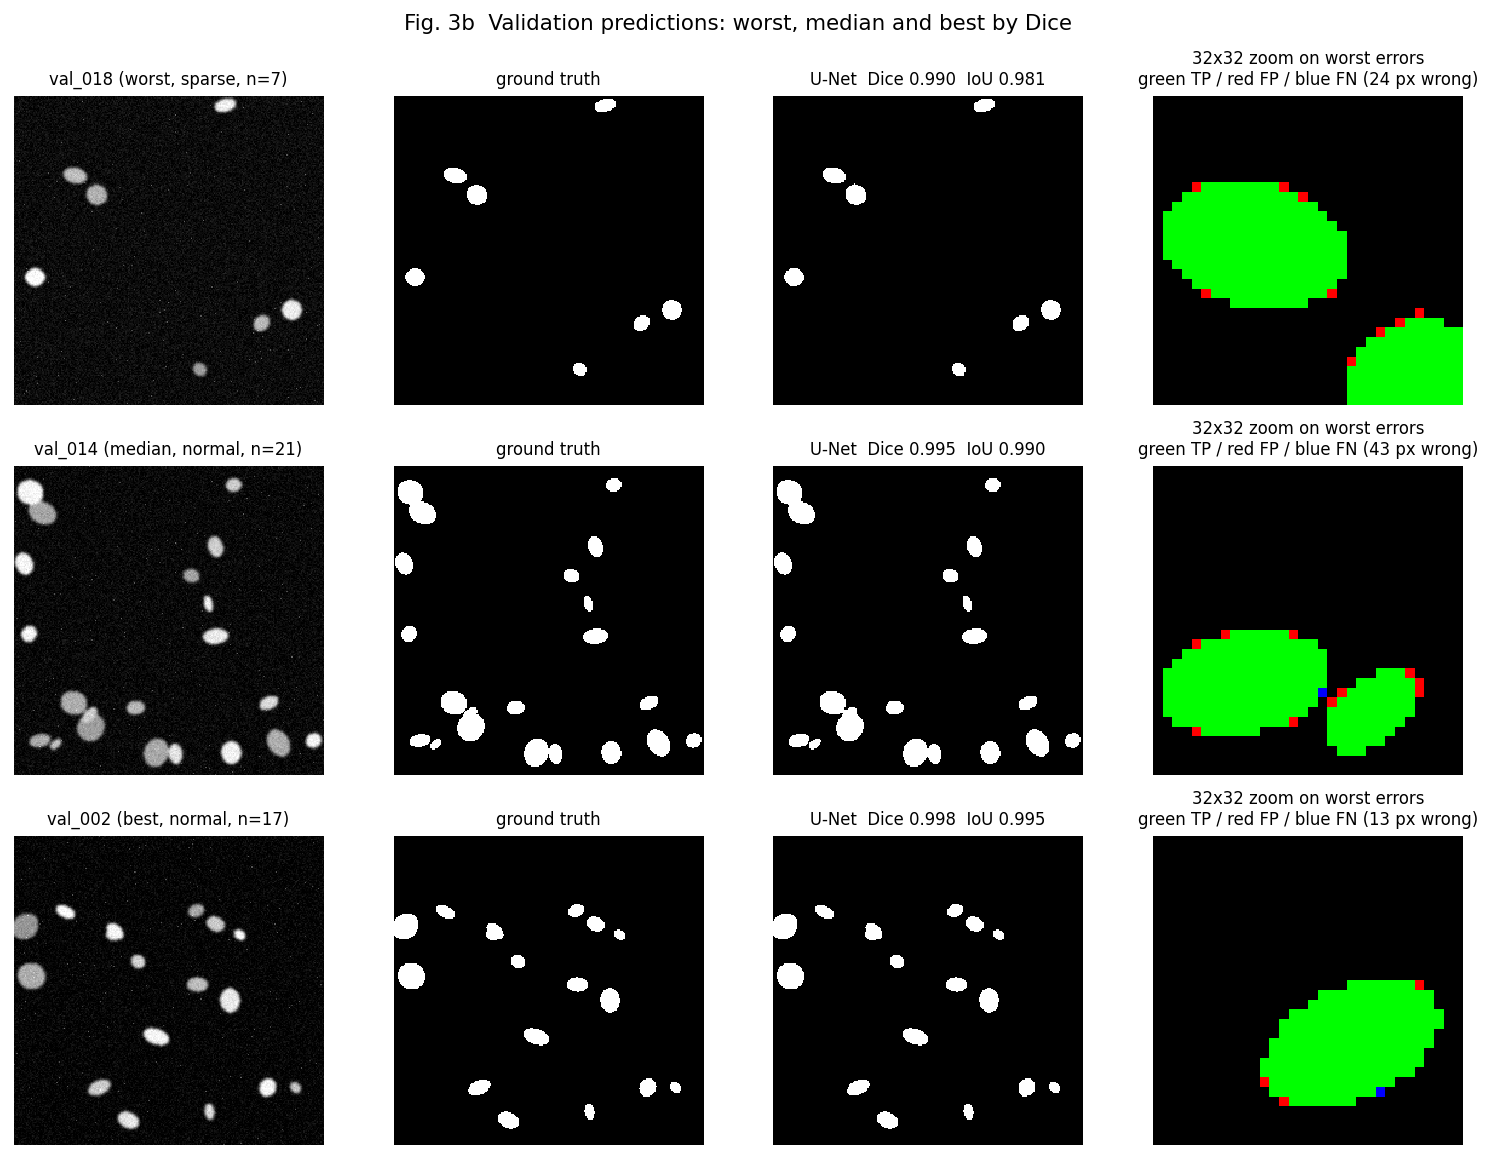
\includegraphics[width=0.56\textwidth]{../results/figures/fig3b_panels.png}
\caption{Input, ground truth, U-Net prediction and a $32\times32$ zoom on the
densest error region, for the worst, median and best validation images by Dice.
At full field size the errors are invisible; the zoom shows that they are almost
entirely a one- to two-pixel band on object boundaries, plus the narrow bridges
where two nuclei touch.}
\end{figure*}

Mean validation Dice was \textbf{0.9946} and mean IoU \textbf{0.9893} --- an
improvement of $+0.021$ Dice over Otsu, and the U-Net won on \textbf{20/20}
individual images. Performance is remarkably flat across regimes; the weakest
group is \textit{sparse} (0.9921), not the clustered images, because with only
5--9 nuclei per image a fixed number of misclassified boundary pixels is a
larger fraction of a small denominator. Dice on small objects is
mechanically harsher, which is a property of the metric rather than of the model
\cite{maierhein2024}.

\begin{figure}[t]
\centering
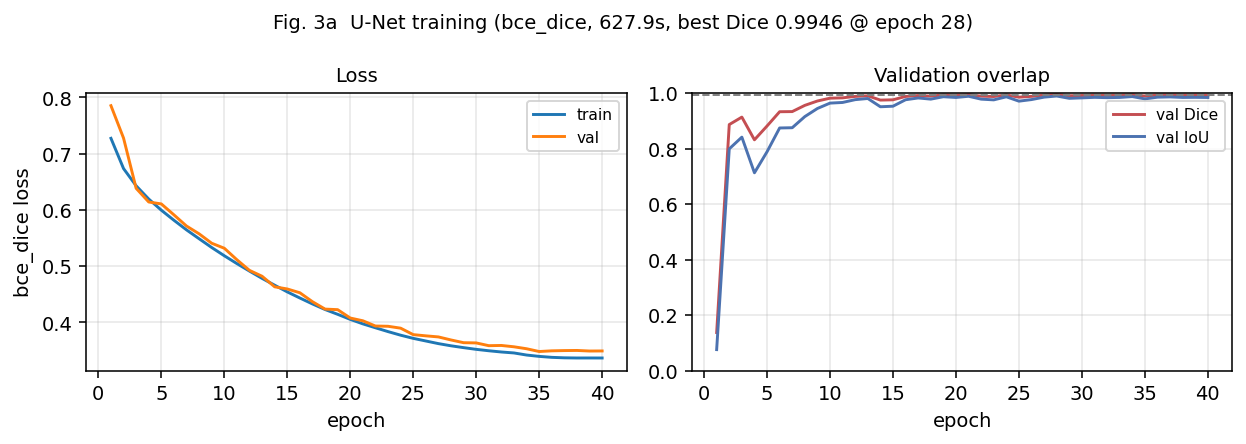
\includegraphics[width=\linewidth]{../results/figures/fig3a_curves.png}
\caption{Training and validation loss, and validation Dice/IoU. Validation Dice
exceeds 0.97 by epoch 9 and then plateaus; train and validation loss track each
other closely, so the model is not overfitting despite the 80-image training
set.}
\end{figure}

The loss curves plateau near 0.34 rather than falling to zero, which looks like
under-training but is not. Soft Dice is computed on \textit{probabilities}: the
network leaves roughly $p{\approx}0.09$ of background probability spread over
$\sim$65{,}000 background pixels, which contributes a large denominator to the
soft-Dice term while costing nothing after thresholding at 0.5. Thresholded Dice
is 0.995 for the same image whose soft-Dice loss is 0.90. This is a useful
reminder that the training objective and the reported metric are not the same
quantity, and that a plateauing loss curve is not by itself evidence of a
problem.

\begin{figure}[t]
\centering
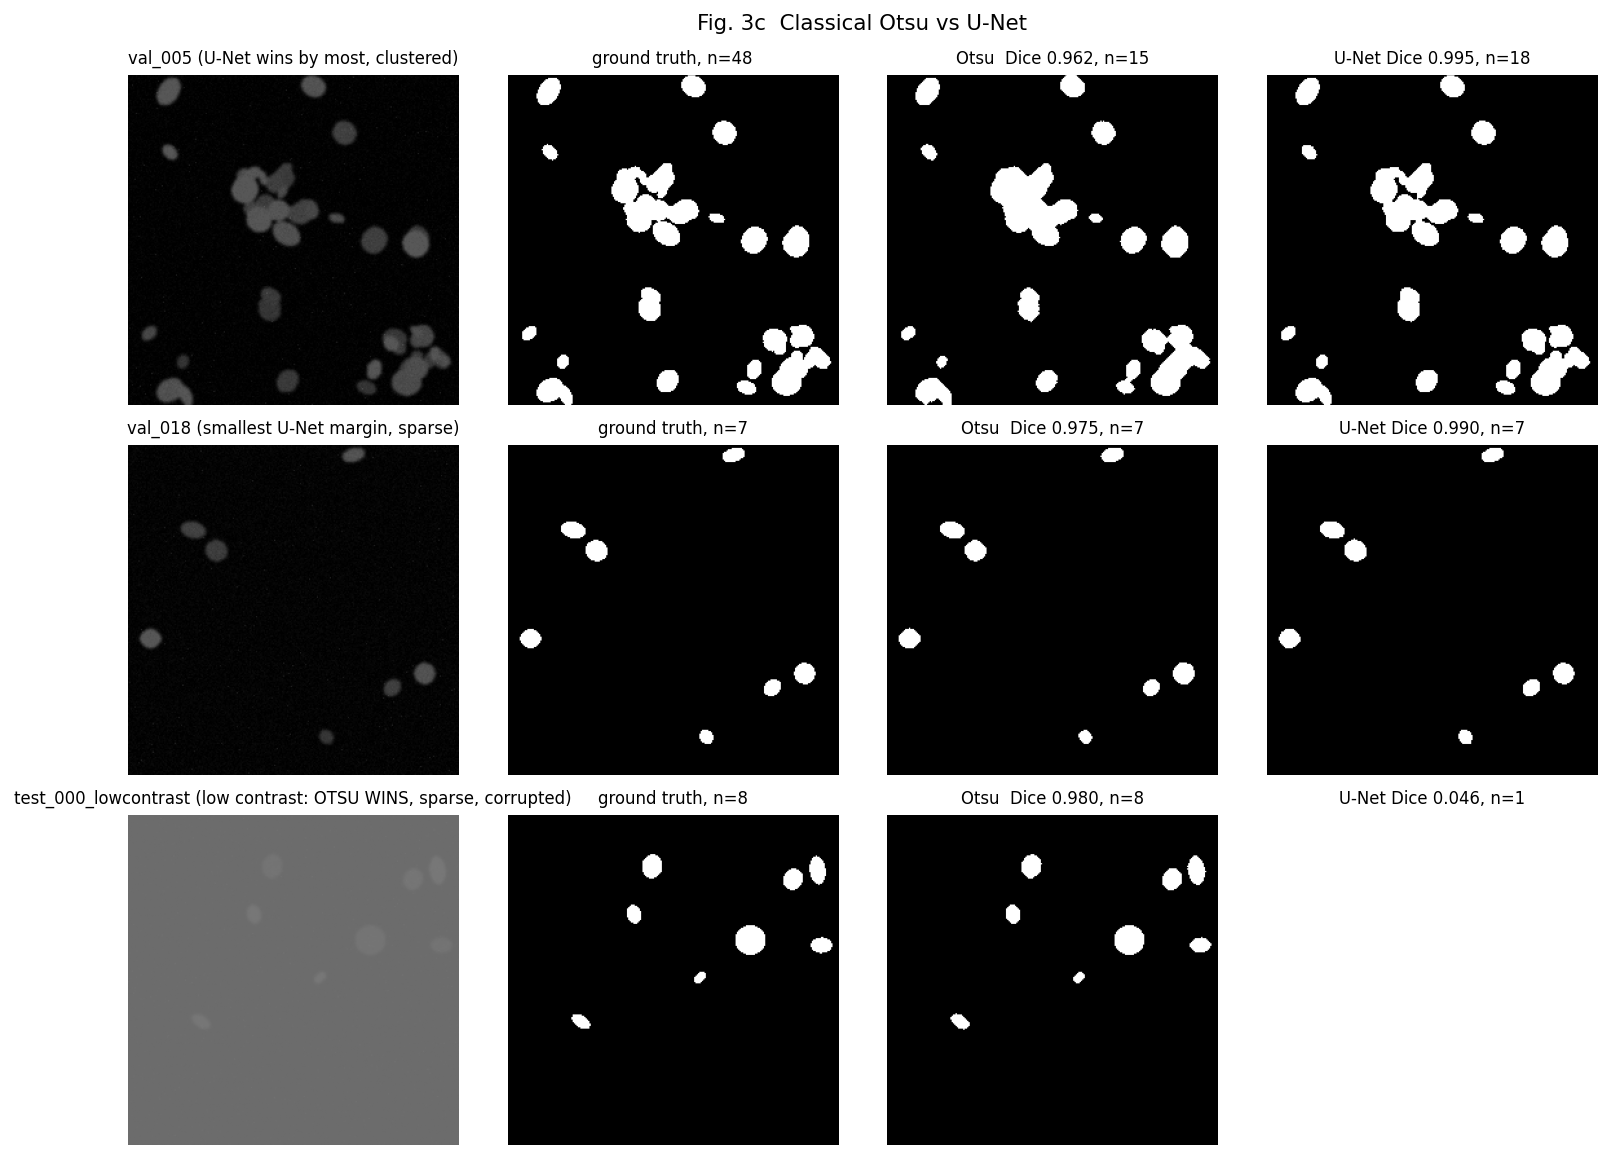
\includegraphics[width=0.95\linewidth]{../results/figures/fig3c_otsu_vs_unet.png}
\caption{Otsu vs U-Net. Top: the largest U-Net margin (\texttt{val\_005},
clustered, Dice 0.962 $\rightarrow$ 0.995) --- the U-Net keeps the thin dark
gaps between touching nuclei that Otsu floods. Middle: the smallest margin
(\texttt{val\_018}, sparse). Bottom: the one regime where \textbf{Otsu wins
decisively} --- a low-contrast acquisition, where Otsu scores 0.980 and the
U-Net collapses to 0.046.}
\end{figure}

\section{Task 4 --- the hybrid pipeline}

The full pipeline was run on the 12 unseen test images: image $\rightarrow$
grayscale $\rightarrow$ U-Net mask $\rightarrow$ debris filter $\rightarrow$
\texttt{regionprops\_table} $\rightarrow$ 14-number evidence block $\rightarrow$
local LLM $\rightarrow$ structured JSON + one-paragraph narrative $\rightarrow$
audit $\rightarrow$ row in a \texttt{pandas} DataFrame, saved as
\texttt{results/task4\_records.csv}.

\begin{prompt}{Optimised hybrid prompt (Task 4, abridged)}
\scriptsize\ttfamily
You are the reporting stage of an automated microscopy pipeline. The
segmentation and the measurements have already been made by code; your only job
is to restate them faithfully in JSON and in one short paragraph. You have NOT
seen the image. Never add a finding, a colour, a diagnosis or a number that is
not in the evidence below, and never change a number that is given to
you.\\[2pt]
EVIDENCE (image\_id=\{image\_id\}) \{summary\}\\[2pt]
Classification rules (apply literally): [density\_class and quality\_flag rules,
identical to Task 2]\\[2pt]
Respond with EXACTLY two parts and nothing else:\\
JSON:\\
\{"image\_id": "\{image\_id\}", "n\_objects": <int>, "mean\_area": <float, 1
decimal place>, "density\_class": "<sparse|normal|dense|clustered>",
"quality\_flag": "<ok|review>"\}\\
NARRATIVE:\\
<one paragraph, 3-5 sentences, descriptive only, no diagnosis, quoting the
counts and areas above. End with the sentence: "Automated description for
educational use only; not a clinical interpretation.">
\end{prompt}

\textbf{Example record and narrative} (\texttt{test\_006}):

{\footnotesize\ttfamily\{"image\_id": "test\_006", "n\_objects": 8,
"mean\_area": 200.0, "density\_class": "sparse", "quality\_flag": "ok"\}}

\begin{quote}\footnotesize
Segmentation of test\_006 produced 8 connected objects occupying 0.024 of the
$256\times256$ field, which the pipeline classes as `sparse'. Mean object area
is 200.0\,px (range 77--318\,px), and mean solidity is 0.966. Objects are
compact and near-circular with mean eccentricity 0.61; where solidity falls
below 0.95 the object may be a merger of touching nuclei rather than a single
one, which is uncertain from these measurements alone. The quality flag is
`ok'. \textit{Automated description for educational use only; not a clinical
interpretation.}
\end{quote}

Every field the pipeline can compute is recomputed after the model replies and
compared to the returned JSON; any disagreement is overwritten by the measured
value and logged in a \texttt{repairs} column, so a malformed or hallucinated
reply degrades to the measurement rather than corrupting the record.

\textbf{Results.} Mean test Dice was 0.9942 and IoU 0.9885 --- indistinguishable
from validation, so the model generalises to the unseen split, and total nuclear
area is accurate to 0.7\%. The record-level numbers tell a different story.
Object count was biased by $-11.9$ per image (MAPE 25.3\%) and
\texttt{density\_class} matched the dataset's own regime label on only 9/12
images. The disagreements all run one way: \texttt{test\_005} (49 nuclei,
\textit{clustered}) was reported as 16 objects and \textit{normal};
\texttt{test\_004} (75, \textit{dense}) as 43. A distance-transform watershed
split of the same masks halves the error (MAPE 14.0\%) without touching the
segmentation, confirming an \textit{instance}-level limitation of binary masks
rather than a pixel-level failure of the network.

\begin{figure}[t]
\centering
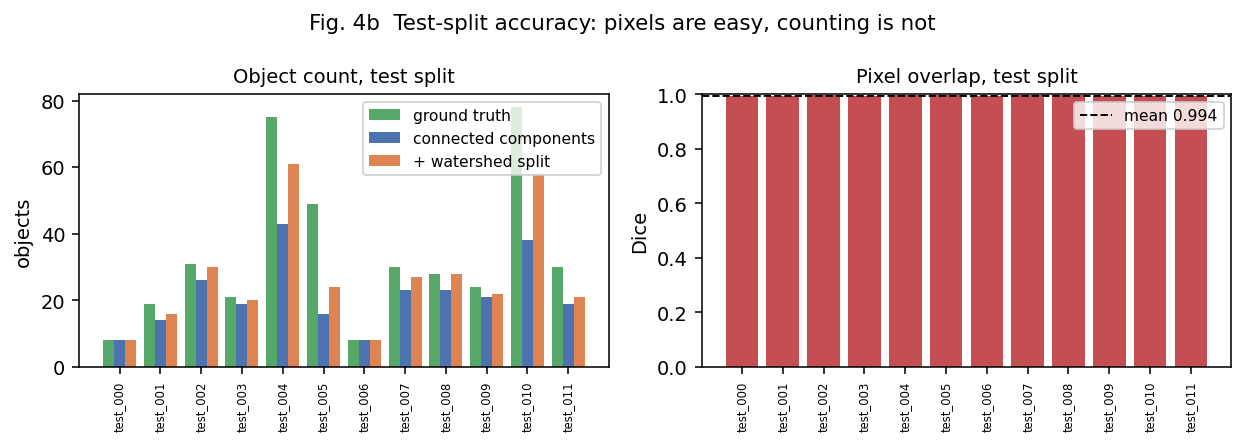
\includegraphics[width=\linewidth]{../results/figures/fig4b_test_metrics.png}
\caption{Test split: object counts (left) and per-image Dice (right). Dice is
above 0.99 everywhere while the count is systematically short --- most severely
on the two \textit{dense} images --- and a watershed split recovers about half
the deficit.}
\end{figure}

\section{Extensions}\label{sec:ext}

\textbf{Robustness.} \texttt{test\_000} was pushed through the pipeline clean and
under three corruptions: the dataset's own heavy-blur and low-contrast variants,
and additive Gaussian noise ($\sigma{=}0.10$) that we generated. Table~2 traces
each stage.

\begin{table}[t]
\centering\scriptsize
\caption{Corruption propagation for \texttt{test\_000} (8 nuclei).}
\begin{tabular}{lcccccc}
\toprule
Variant & px sd & QC & U-Net & Otsu & $n$ & record\\
        &       & flags & Dice & Dice &     & (density/quality)\\
\midrule
clean        & 0.035 & --- & 0.995 & 0.980 & 8 & sparse / ok\\
blur         & 0.020 & \checkmark & 0.651 & 0.671 & 7 & sparse / ok\\
low contrast & 0.005 & \checkmark & 0.046 & 0.980 & 1 & sparse / \textbf{review}\\
noise        & 0.070 & --- & 0.820 & 0.818 & 9 & \textbf{clustered} / ok\\
\bottomrule
\end{tabular}
\end{table}

The interesting question is not whether corruption is detectable but
\textit{where}, and under what information. With the clean image in hand, all
three are visible at stage~1 from pixel statistics alone. Without it --- which is
the deployable case --- three reference-free input checks (dynamic range
$<0.020$, mean $>0.15$, variance of the Laplacian $<2\times10^{-4}$) catch blur
and low contrast at stage~1, and the low-contrast case is caught \textit{again}
at stage~4 because the mask floods the whole field and the foreground fraction
leaves the accepted range, tripping \texttt{quality\_flag = review}. Additive
noise is the dangerous one: it passes every input check, degrades U-Net Dice to
0.82, fragments nuclei so the count rises from 8 to 9, and drives mean solidity
below 0.90, which silently flips \texttt{density\_class} from
\textit{sparse} to \textit{clustered} --- with \texttt{quality\_flag} still
\texttt{ok}. \textbf{The earliest reliably detectable stage for noise is
stage~4, and it manifests as a wrong answer rather than a warning.} A narrative
generated from that record is fluent, internally consistent and wrong.

\textbf{Loss ablation.} The same architecture, schedule and seed were trained
with BCE, soft Dice and BCE+Dice (Table~3). The spread is 0.002 Dice between
best and worst, which on a 20-image validation split we would not defend as
significant: the task is close to separable and all three objectives find
essentially the same solution. The one systematic effect is in the tail. Pure
soft Dice has the worst worst-image score (0.9771 against 0.9902 and 0.9906) and
peaks earliest, at epoch 21. Soft Dice normalises by a per-image foreground
denominator, so on \textit{sparse} images (2\% foreground) a few pixels swing
the loss and the gradient is noisy; BCE is stable but its gradient is dominated
by the $\sim$92\% of trivially easy background. The sum inherits BCE's
stability and Dice's region-level signal, which is why it wins and why its
margin is largest where the foreground is smallest.

\begin{table}[t]
\centering\footnotesize
\caption{Loss ablation, 40 epochs, validation split.}
\begin{tabular}{lcccc}
\toprule
Loss & mean Dice & mean IoU & worst image & best epoch\\
\midrule
%%ABLATION%%
\bottomrule
\end{tabular}
\end{table}

\textbf{Intensity-robust training.} The low-contrast collapse in Table~2 is a
distribution-shift failure, not a capacity failure: every training image shares
one intensity scale, so the network learned an absolute-brightness decision rule
where Otsu uses a relative one. Retraining with per-image percentile contrast
normalisation (1st/99.5th $\rightarrow$ 0/1) plus photometric augmentation
(random gain 0.25--1.75, offset, blur and noise) tests that explanation
directly.

%%ROBUSTTRAIN%%

\begin{figure}[t]
\centering
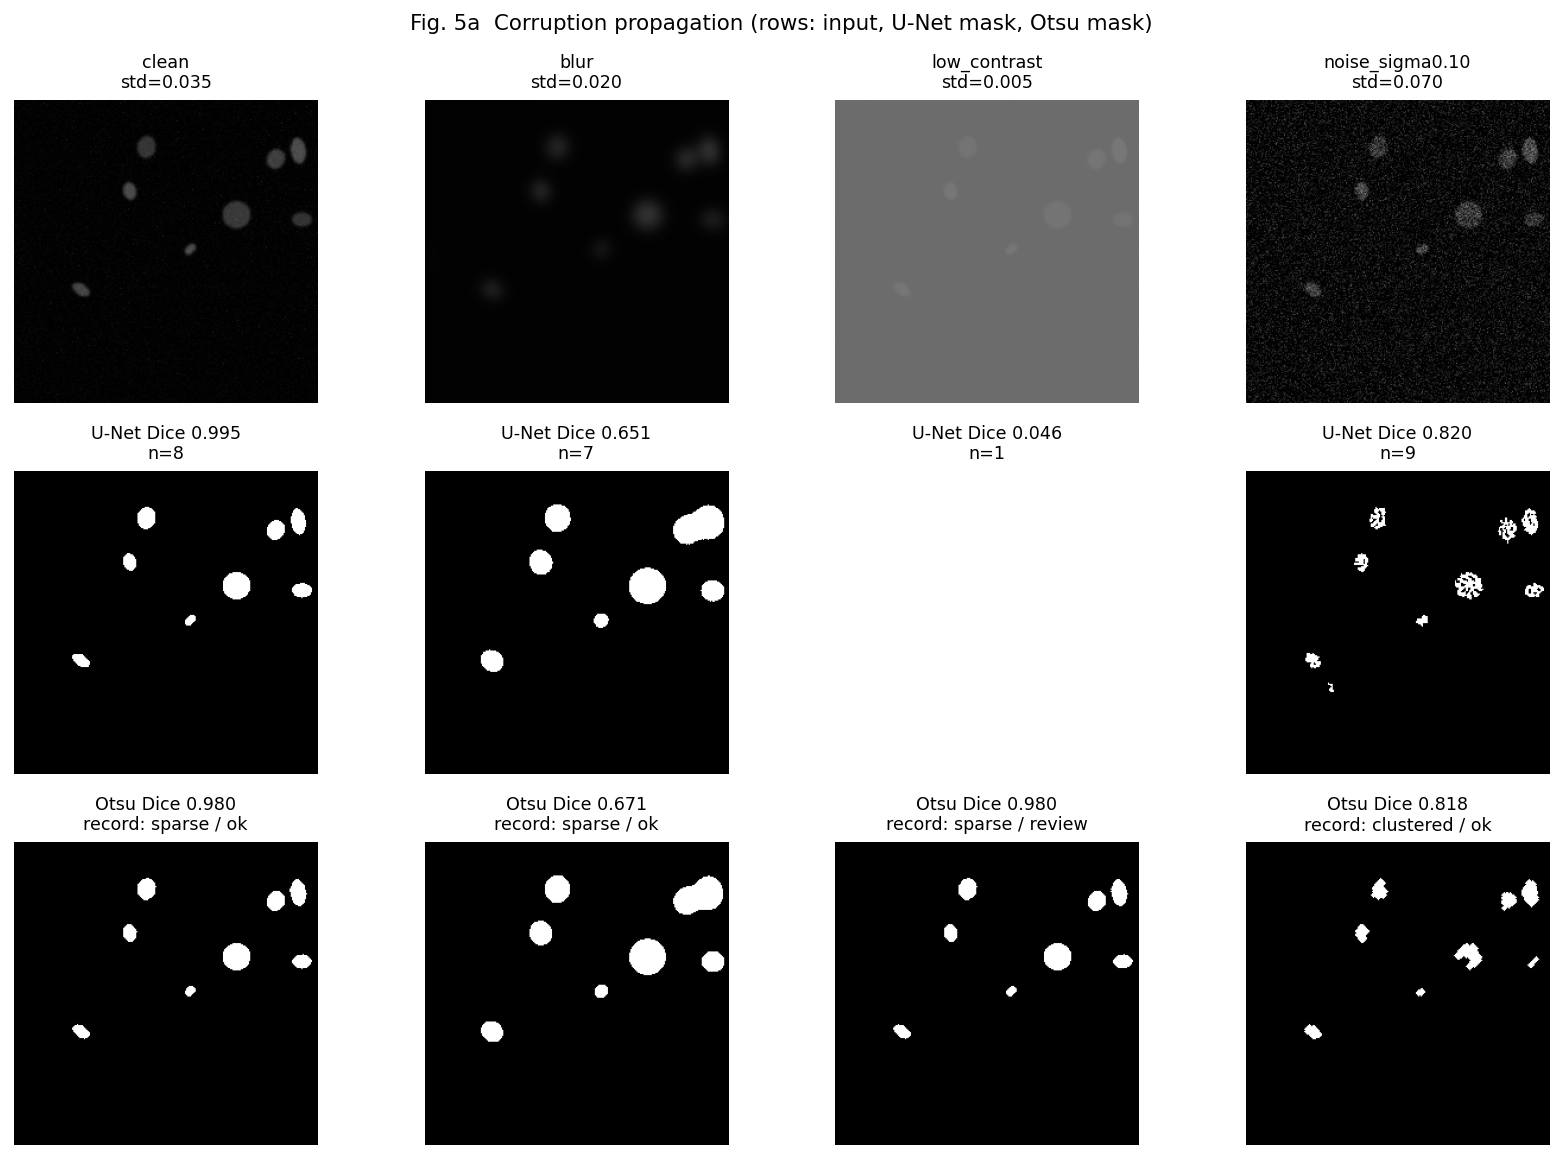
\includegraphics[width=0.70\linewidth]{../results/figures/fig5a_robustness.png}
\caption{Corruption propagation. Rows: input, U-Net mask, Otsu mask. Under low
contrast the U-Net labels the entire field as foreground (one 65{,}536\,px
``object'') while Otsu is unaffected, because Otsu re-derives its threshold from
each image.}
\end{figure}

\begin{figure}[t]
\centering
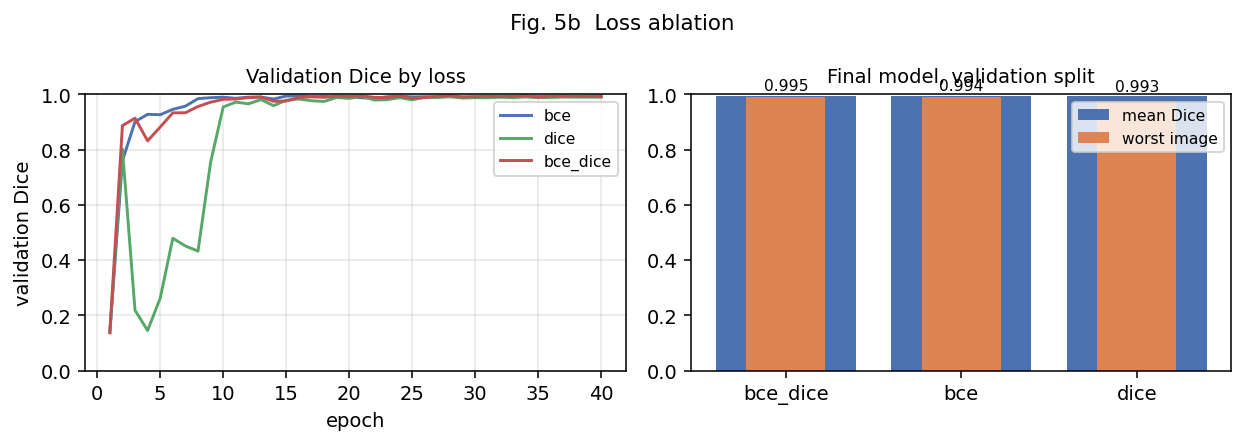
\includegraphics[width=0.74\linewidth]{../results/figures/fig5b_loss_ablation.png}\\[1pt]
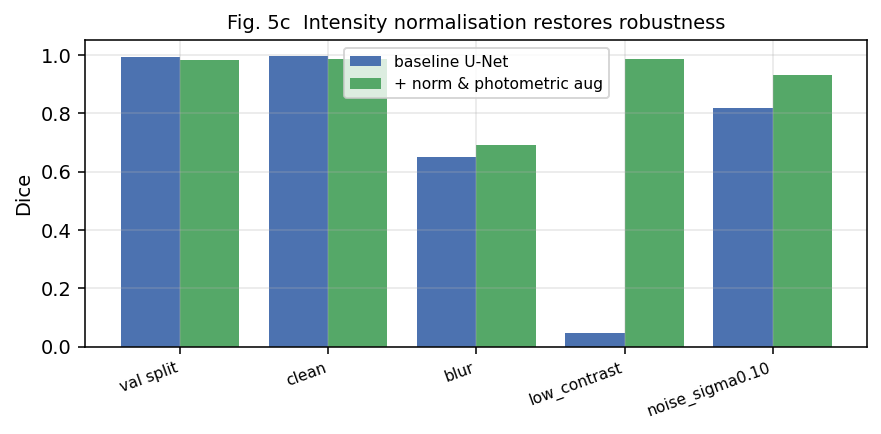
\includegraphics[width=0.54\linewidth]{../results/figures/fig5c_robust_training.png}
\caption{Top: validation Dice per epoch for the three losses, and final mean /
worst-image Dice. Bottom: baseline U-Net versus the same network trained with
percentile normalisation and photometric augmentation, on the clean validation
split and the three corruptions.}
\end{figure}

\section{Discussion --- the five questions}

\textbf{1. Which description is more useful, and which more trustworthy?}
They are not the same axis. The direct VLM description (Task~1) is more
\textit{useful} in the narrow sense that it is the only stage that can report
something nobody thought to measure --- a smear, a folded edge, a second
fluorophore --- because it looks at pixels rather than at a fixed 14-number
vector. It is by far the less \textit{trustworthy}: it produced no parseable
JSON under a naive prompt, gave three different answers to the same question in
three runs, and volunteered a clinical inference (``hyperproliferative
process'') that the image cannot support. The numbers-first description
(Task~2) is trustworthy in a specific, checkable sense: every quantity in it was
computed by \texttt{regionprops}, and we checked them against ground truth: total
nuclear area is accurate to 0.7\% on the test split, while the object
\emph{count} is 25\% short.
Its failure mode is the opposite of the VLM's --- it is confidently wrong
whenever the measurement is wrong, and it cannot notice, because it never saw
the image. They are complementary: numbers for anything aggregated or acted on, VLM for
open-ended triage of what the schema does not cover, and neither alone.

\textbf{2. Did the U-Net improve on Otsu?} On clean data, yes and
uniformly: 0.9946 vs 0.9733 mean Dice, winning 20/20 validation images. The
clearest win is \texttt{val\_005} (clustered, 48 nuclei), 0.962 $\rightarrow$
0.995: Otsu floods the one- to two-pixel dark gaps between touching nuclei
because those pixels sit below its global threshold, while the U-Net has learned
the local shape context that keeps the gap open (Fig.~5, top). The clearest
\textbf{Otsu} win is the low-contrast \texttt{test\_000} variant, where Otsu
scores 0.980 and the U-Net 0.046 (Fig.~5, bottom). Otsu recomputes its threshold
from each image's own histogram and is therefore invariant to affine intensity
rescaling; the U-Net saw exactly one intensity regime in training and had no
reason to learn that invariance. The U-Net is better on the distribution it was trained on and much worse off
it --- the generic trade-off between a learned prior and a per-image statistic.

\textbf{3. Dice and IoU, and where the mistakes are.} Validation Dice 0.9946,
IoU 0.9893; test Dice 0.9942, IoU 0.9885. Dice is
$2|P\cap G|/(|P|+|G|)$ and IoU is $|P\cap G|/|P\cup G|$; both are pure
\textit{pixel-overlap} measures, so 0.9946 means about half a percent of
foreground-or-predicted pixels are on the wrong side. The zoom panels in Fig.~3
localise them: they are a one- to two-pixel band around object boundaries plus
the bridges where nuclei touch. Two caveats matter more than the
headline number: the metric is hardest on sparse images (0.9921) purely because
the denominator is small, and --- far more importantly --- these numbers say
almost nothing about whether the pipeline is right, since the same masks
under-count nuclei by 25\% and mis-class density on 25\% of test images. Pixel
overlap is the wrong metric for a task whose output is a count
\cite{maierhein2024,caicedo2019}.

\textbf{4. Where can the LLM hallucinate, and what reduces the risk?} Three
places. (a) Task~1, where it sees an image and can invent anything --- observed
here as unsupported diagnostic language. (b) Task~2/4 JSON, where it can copy a
number wrongly, invent a field or emit a value outside the allowed set. (c) The
narrative, where it can add a clause the evidence does not license. The
mitigations are, in order of effect: give the model no image at the reporting
stage, so there is nothing to hallucinate \textit{from}; move every threshold
into the prompt as a literal rule so the model formats rather than judges;
constrain each field to a closed vocabulary; require an explicit
\texttt{uncertain}; and then \textbf{recompute every computable field in code
and overwrite disagreements}, logging them. Keeping the structured JSON as the source of truth is the
difference between a system you can audit and one you can only read: JSON is
diff-able across runs, aggregable, checkable against ground truth and traceable
to a specific mask and feature table, whereas a paragraph is none of those. Our
repair layer fired 0 times; its value is not the count but that a non-zero count
would be \textit{visible} rather than silent.

\textbf{5. Would I trust any of it clinically?} No part of it, and the reasons are not
fixable by more epochs. The dataset is synthetic and seeded, so the near-perfect
Dice measures how well a small U-Net fits an easy, noise-free forward model, not
how it would handle real tissue with out-of-focus planes, autofluorescence,
debris and genuinely overlapping nuclei. With 20 validation and 12 test images,
a Dice quoted to four decimals has a confidence interval far wider than the
differences discussed here. The system has no calibrated uncertainty, was
evaluated on one modality, and --- as the noise experiment shows --- fails
silently rather than loudly. The one component with a defensible claim to trust
is the audit trail: each record is reproducible from a seed, a checkpoint and a
logged prompt, and LLM/measurement disagreements are recorded.

If I could make a single change, it would be to \textbf{replace pixel
segmentation with instance segmentation and report a calibrated count with an
abstention rule} --- concretely, a watershed or a StarDist/Cellpose-style
instance head \cite{schmidt2018,stringer2021} whose output is validated against
instance-level metrics (per-object F1 at matched IoU), with the pipeline
refusing to emit a record when the input QC checks or the predicted uncertainty
exceed a threshold. That single change attacks the largest observed error (the
25\% under-count), replaces the metric that currently flatters the system, and
converts the noise failure from a wrong answer into a refusal --- which is the
only failure mode that is safe in a clinical workflow.

\section*{Limitations and provenance}
The LLM text quoted above came from the offline stub (box, Section~2): it
demonstrates the pipeline's contract --- schema, audit, repair --- not the
behaviour of \texttt{llama3.2-vision} specifically, and re-running the scripts
against Ollama replaces those artefacts in place. Every other number and figure
is a real measurement on the assigned dataset, written by the code in the
accompanying repository (\texttt{run\_all.sh} reproduces them end to end). All
outputs are educational only; nothing here is cleared for clinical use.

{\scriptsize
\bibliographystyle{unsrt}
\begin{thebibliography}{9}
\setlength{\itemsep}{-1pt}\setlength{\parskip}{0pt}
\bibitem{ronneberger2015} O.~Ronneberger et al. U-Net: Convolutional Networks
for Biomedical Image Segmentation. \textit{MICCAI}, 2015.
\bibitem{otsu1979} N.~Otsu. A Threshold Selection Method from Gray-Level
Histograms. \textit{IEEE Trans. SMC}, 9(1):62--66, 1979.
\bibitem{maierhein2024} L.~Maier-Hein et al. Metrics reloaded. \textit{Nature
Methods}, 21:195--212, 2024.
\bibitem{caicedo2019} J.~C.~Caicedo et al. Nucleus segmentation across imaging
experiments. \textit{Nature Methods}, 16:1247, 2019.
\bibitem{schmidt2018} U.~Schmidt et al. Cell Detection with Star-convex
Polygons. \textit{MICCAI}, 2018.
\bibitem{stringer2021} C.~Stringer et al. Cellpose: a generalist algorithm for
cellular segmentation. \textit{Nature Methods}, 18:100--106, 2021.
\bibitem{ji2023} Z.~Ji et al. Survey of Hallucination in Natural Language
Generation. \textit{ACM Comput. Surv.}, 55(12):1--38, 2023.
\end{thebibliography}
}

\end{document}
